\documentclass[12pt]{article}
\usepackage[a4paper, left = 24mm, top = 24mm, bottom = 24mm, right = 24mm]{geometry}
\usepackage{amsfonts, amsmath, amssymb}
\usepackage{gensymb}
\usepackage{fancyhdr}
\usepackage{pdfpages}
\usepackage{listings}
\usepackage{color}
\usepackage{pdfpages}
\usepackage{hyperref}
\usepackage{verbatim}
\usepackage[utf8]{inputenc}
\usepackage{graphicx}
\usepackage{float}
\usepackage{longtable}
\usepackage{fontenc}
\usepackage[backend=biber, style=ieee]{biblatex}
\usepackage{fontenc}
\usepackage{times}
\usepackage[ddmmyyyy]{datetime}
\usepackage{pdfpages}
\usepackage{subcaption}

\setlength{\parindent}{0pt}
\setlength{\parskip}{1em}

%\addbibresource{biblo.bib}

\pagestyle{empty}

\begin{document}

\title{ELEC3208 Design Exercise CW FM Radar}
\author{Peter Alexander - 29462878}

\maketitle

\newpage
\tableofcontents
\newpage

% Content 
\section{System Block Diagram}
\label{sec:System Block Diagram}

Figure \ref{fig:systemBlockDiagram} shows the system block diagram that was implemented for this project. 
It has been split into subsections each serving a particular function.
The 8-Bit digital output of the system is sent to the microcontroller at the bottom right of the diagram. 

\begin{center}
    \begin{figure}[H]
        \includegraphics[width=0.9\textwidth]{../BlockDiagram/systemBlockDiagram.png}
        \caption{A figure showing the system block diagram from which the system described in this report was designed}
        \label{fig:systemBlockDiagram}
    \end{figure}
\end{center}

\subsection{Operational Principles}
A periodic signal, in this case a triangle wave, is modulated onto an ultrasonic carrier to produce an FM-modulated signal that is emitted by an ultrasonic transducer.
This signal propagates through the air at the speed of sound (344 m/s at sea level under normal conditions) and reflects off of any solid objects in its path. 
This reflection is converted back to an electrical signal by a second transducer.

A PLL with a center frequency equal to that of the FM modulator is used to demodulate the signal. 
The output of the loop filter will vary with the frequency of the incoming signal, accurately following the triangle wave generated in the Modulation stage. 
The reconstructed triangle wave is then compared with the wave generated at that instant. 
The potential difference between the signals is directly proportional to the time it took for the reconstructed signal to travel to and from the object off of which it reflected.
The distance from the transducers to the reflecting surface can be calculated from this potential difference. 

Below is a description of the function of each subsection and an outline of the function of each block from the practical system in Figure \ref{fig:systemBlockDiagram}. 

\subsection{Modulation}
The triangle wave is generated in the Triangle Wave Generator.
It is used as the input to the VCO with a center frequency set at 40KHz. 
The bandwidth of the FM signal is specified in the tuning sensitivity ($K_{VCO}$) of the VCO.
As the parameters of the transducers are not known, an optional transmission amplifier has been included.
On a PCB, a jumper could be used to bypass the transmission amplifier if the VCO proved suitably powerful. 
The PCB area for the transmission amplifier would only be populated if required. 

%
\section{Specification}
\label{sec:specification}

\subsection{System-Wide Specification}
\label{sec:systemWideSpecification}
The system should run on $\pm$ 5 V as the robot will likely have a central PSU that provides this configuration.
As stated in the specification, the maximum measurable distance $d_{max}$ should be 5 m. 
The distance measurement is converted into an 8-Bit word so the minimum measurable distance $d_{min}$ should be given by Equation \eqref{eqn:minimumMeasurableDistance}
\
\begin{align}
    \begin{split}
        d_{min} & =  \frac{5\ m}{2^8-1}\\
                & =  \frac{5\ m}{255}\\
                & =   2.0\ cm
    \end{split}
    \label{eqn:minimumMeasurableDistance}
\end{align}

To get accurate results, the triangle waves measured by the differential amplifiers must have a phase difference of no more than \(\pi\) radians at the maximum measurable value of 5 m.
To reduce the time spent in the latched state (where the two signals are moving in opposite directions) the phase difference at maximum range will be reduced to \(\frac{2}{3}\pi\). 
With the speed of sound at sea level under normal conditions $V_{s}$ equal to 344 m/s, the total propagation delay $t_{p}$ imposed on the reflected signal given by Equation \eqref{eqn:propagationDelay}.
This is \(\frac{1}{3}\) of the total triangle wave period $T$. 
This gives T as 87.3 ms and a frequency F of 11.5 Hz.

\begin{align}
    \begin{split}
        t_{p} & = 2\frac{d_{p}}{V_{s}}\\
              & = 2\frac{5\ m}{344\ m/s}\\
              & = 29.1\ ms
    \end{split}
    \label{eqn:propagationDelay}
\end{align}

A maximum frequency variation $\Delta f$ of 4 kHz, resulting in a bandwidth of 8 kHz, was chosen as a compromise between simpler filter/amplifier design requiring high bandwidth, and the use of more cost-effective VCO and PLL elements requiring lower bandwidth.  

\subsection{Modulation Section Specification}

\subsubsection{Triangle Wave Generator}
\label{sec:specificationTriangleWaveGenerator}
\begin{itemize}
    \item \textbf{Frequency} - 11.5 Hz $\pm$ 1 Hz to match the system spec in Section \ref{sec:systemWideSpecification}. The theoretical maximum of this value is 17.2 Hz, beyond this value the two triangle waves will be more than $\pi$ radians out of phase when measuring 5 m and the digital output would be in the lathed state 50\% of the time.
    \item \textbf{Amplitude} - 1 V $\pm$ 0.05 V as a compromise between low power operation and low $K_{VCO}$.
    \item \textbf{Offset} - 0 V $\pm$ 0.1 V to ensure center frequency at 40 kHz. 
    The tolerance of the offset and amplitude values are to limit variations in the bandwidth of the FM signal.
\end{itemize}

\subsubsection{VCO}
\label{sec:specificationVCO}
\begin{itemize}
    \item \textbf{Center Frequency} 40 kHz $\pm$ 200 Hz. Low tolerance offset error on PLL output is minimised
    \item \textbf{$K_{VCO}$} - KVCO of 4 kHz/V $\pm$ 500 Hz as calculated in Equation \eqref{eqn:KVCO}.

    \begin{equation}
        \begin{split}
             K_{VCO} &= \frac{f_{max} - f_{min}}{V_{max} - V_{min}}\\
                     &= \frac{44 kHz - 36 kHz}{1V - -1V} = 4 kHz/V
        \end{split}
        \label{eqn:KVCO}
    \end{equation}
\end{itemize}

\subsubsection{Transmission Amplifier}
\label{sec:specificationTransmissionAmplifier}
A MOSFET should be used to amplify the square wave produced by the VCO.
An engineer should be able to set the fabricated PCB into two configurations:
\begin{enumerate}
    \item \textbf{VCO $\rightarrow$ Transducer} - The output of the VCO is fed into the positive terminal of the transducer.
    The negative terminal of the transducer is set to ground. 
    \item \textbf{VCO $\rightarrow$ MOSFET Gate} - The output of the VCO is fed into the Gate of an N-channel MOSFET. The positive terminal of the transducer is connected to 5V or an external voltage supply.
    The negative terminal of the transducer is connected to the drain of the MOSFET.
\end{enumerate}
The MOSFET should have the following parameters:
\begin{itemize}
    \item \textbf{Voltage Rating} - 20 V, higher voltages could prove dangerous for engineers working with the hardware.
    \item \textbf{Current Rating} - 1A, electroacoustic transducers are capacitive devices so current requirements are relatively low. 
\end{itemize}

\subsection{Demodulator Specification}

\subsubsection{Pre-amp}
\label{sec:specificationPreAmp}
As nothing is known about the transducers to be used on the system, few of the amplifier parameters can be specified.
However, the following criteria can be specified:
\begin{itemize}
    \item \textbf{Gain Selection} - The gain of the amplifier should easy to set using commonly available passive components
    \item \textbf{Gain Range} - The gain should be selectable between a factor of 2 and a factor of 2000.
    \item \textbf{Bandwidth Stability} - Setting the gain between 2 and 200 should not reduce the gain in the range of 3500 kHz to 45 kHz by more than 3 dB.
\end{itemize} 

\subsubsection{PLL}
\label{sec:specificationPLL}
\begin{itemize}
    \item \textbf{Centre Frequency} - 40 kHz $\pm$ 200 Hz to match that of the VCO.
    \item \textbf{Triangle Wave Output Offset} - 0V $\pm$ 0.1V to minimise systematic error at the differential amplifier.
    \item \textbf{Amplitude} 1 V $\pm$ 0.1 V to match that of the triangle wave generator.
    If necessary, this should be achieved with an additional amplifier. 
\end{itemize}

\subsection{Analogue to Digital Conversion}

\subsubsection{Differential Amplifier}
\label{sec:specificationDifferentialAmp}
Parameters for the differential amplifier rely on the parameters of the ADC so they shall be described as such. 
\begin{itemize}
    \item \textbf{Differential Gain} - A potential difference of 0.33 V, corresponding to the maximum phase difference between the triangle waves of $\frac{2}{3}\pi$ radians should result in the output of the ADC reaching the upper limit of the ADC input range $V_{ADC} \pm \frac{1}{2^{8}-1}V_{ADC}$.
    This is so the phase difference caused by the transmitted wave reflecting off an object 5 m away generates the maximum value on the ADC.
    
    \item \textbf{Rectified Output} - The polarity of the inputs will periodically switch as the triangle waves change direction.
    The output of the amplifier should include a full-wave rectifier with a lower limit below $\frac{1}{2^{8}-1}V_{ADC}$ so the minimum distance can still be measured.
\end{itemize}

\subsubsection{Differentiator}
\label{sec:specificationDifferentiator}
\begin{itemize}
    \item \textbf{Single Supply} - The output of the differentiators are used as the inputs to digital circuits so their output should not go below 0 V.

    \item \textbf{Gain} - The required gain can be calculated by first finding the minimum rate of change of the triangle wave and finding the minimum multiplier that results in an output meeting the TTL logic HIGH/LOW levels.
    The rate of change is calculated in Equation \ref{eqn:triangleWaveRateOfChange}.
    \begin{equation}
        \begin{split}
            Rate Of Change  &= \frac{Peak-to-Peak Voltage}{\frac{1}{2}*Maximum Period}\\
                            &= \frac{1 V - -1V}{\frac{1}{2}*95.3 ms}\\
                            &= 42.0 V/s
        \end{split}
        \label{eqn:triangleWaveRateOfChange}
    \end{equation} 

    \citeauthor{TTLLogicLevels} state in \citetitle{TTLLogicLevels} that the logic levels for TTL inputs are $V_{in} < 0.8 V$ for guaranteed logic LOW and $V_{in} > 2 V$ for logic HIGH.
    A gain of 0.5 will suffice.

\end{itemize}
%
\section{Implementation}
\label{sec:implementation}

All simulations have been produced in LTSpice.
Each simulated component is implemented as a hierarchical subcircuit and a testbench is produced to verify that the spec has been met. 

\subsection{Modulation}
\subsubsection{Triangle Wave Generator}
\label{sec:implementationTriangleWaveGenerator}
The topology implemented for this subcircuit was found in \citetitle{TriangleWaveTopology}\cite{TriangleWaveTopology}. 
It uses an integrator to generate a ramp from the output of a non-inverting schmitt trigger. 
This ramp is fed into the input of the schmitt trigger. When the ramp reaches a schmitt trigger threshold, the polarity of the schmitt trigger output reverses, forcing the integrator to ramp in the opposite direction. 
High precision, rail-to-rail opamps and E96 resistors ensure the amplitude and offset tolerances were met. 

Figure \ref{fig:triangleWaveGeneratorSchematic} shows the schematic, and Figure \ref{fig:triangleWaveGeneratorTestBench} shows the testbench used to test it. 
The Spice error log shows the results of the measurement directives.
The offset is 0.003V and the peak-to-peak voltage is 2.001 V.
The steady-state frequency is measured as 11.3532 Hz.
Each of these falls within the tolerances presented in Section \ref{sec:specificationTriangleWaveGenerator}.
A cutting of the waveform produced can be found in Figure \ref{fig:triangleWaveGeneratorWaveform}. 


\begin{figure}[H]
    \centering 
    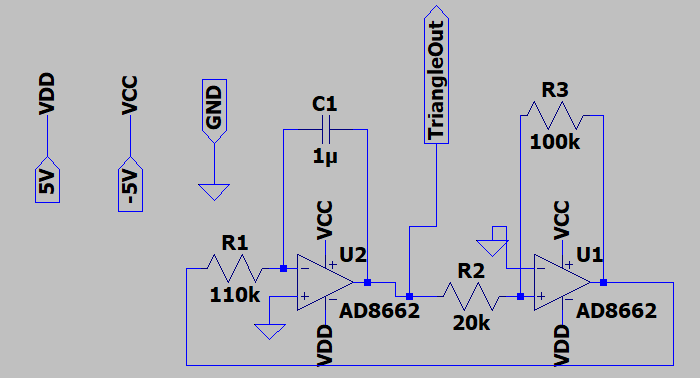
\includegraphics[width=\textwidth]{../Circuits/Images/TriangleWaveGenerator/schematic}
    \caption{A screencap of the Triangle Wave Generator Subcircuit}
    \label{fig:triangleWaveGeneratorSchematic}
\end{figure}

\begin{figure}[H]
    \centering 
    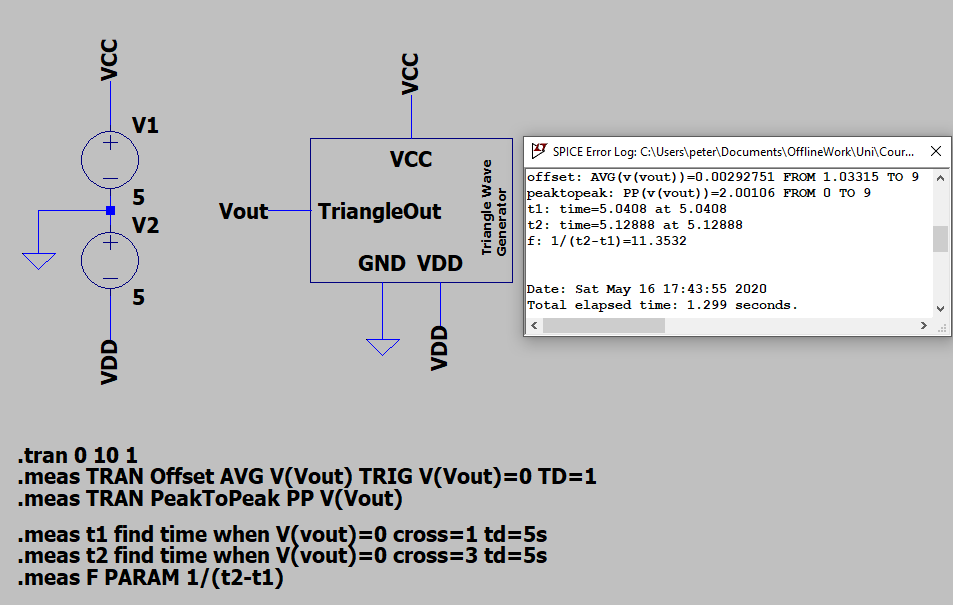
\includegraphics[width=\textwidth]{../Circuits/Images/TriangleWaveGenerator/TestBenchScreencap}
    \caption{A screencap of the Triangle Wave Generator Subcircuit}
    \label{fig:triangleWaveGeneratorTestBench}
\end{figure}

\begin{figure}[H]
    \centering 
    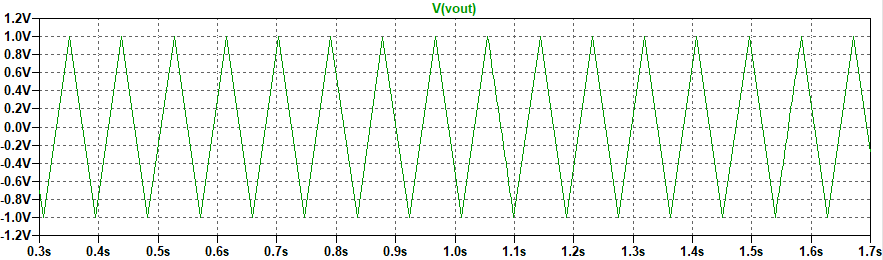
\includegraphics[width=\textwidth]{../Circuits/Images/TriangleWaveGenerator/OutputWaveform}
    \caption{A screencap of the Triangle Wave Generator Subcircuit}
    \label{fig:triangleWaveGeneratorWaveform}
\end{figure}

\subsubsection{VCO}
The VCO subcircuit is based on the LTC6990 VCO IC. 
$K_{VCO}$ and the centre frequency are set using E96 resistors.
The LTSpice schematic was adapted from a circuit generatd automatically on an online design tool provided by Analog Devices\footnote{\url{http://beta-tools.analog.com/timerblox/LTC6990}}.
The schematic is shown in Figure \ref{fig:VCOSchematic}.

The testbench varies the control voltage VC and takes frequency measurements at the appropriate times. 
The testbench is shown in Figure \ref{fig:VCOTestBench}.
The waveform produced is shown in Figure \ref{fig:VCOTestBenchWaveform}.

The measurements showed that the centre` frequency ($F_{Centre}$) is 39842 Hz and the Bandwidth of the FM Modulated signal is 7905.5 Hz.
This falls within the tolerances presented in Section \ref{sec:specificationVCO}.

This IC shifts the phase of the signal by $\pi$ radians, the FM signal frequency increases when VC drops and vica versa. 
The differential amplifier will need to account for this. 

\begin{figure}[H]
    \centering 
    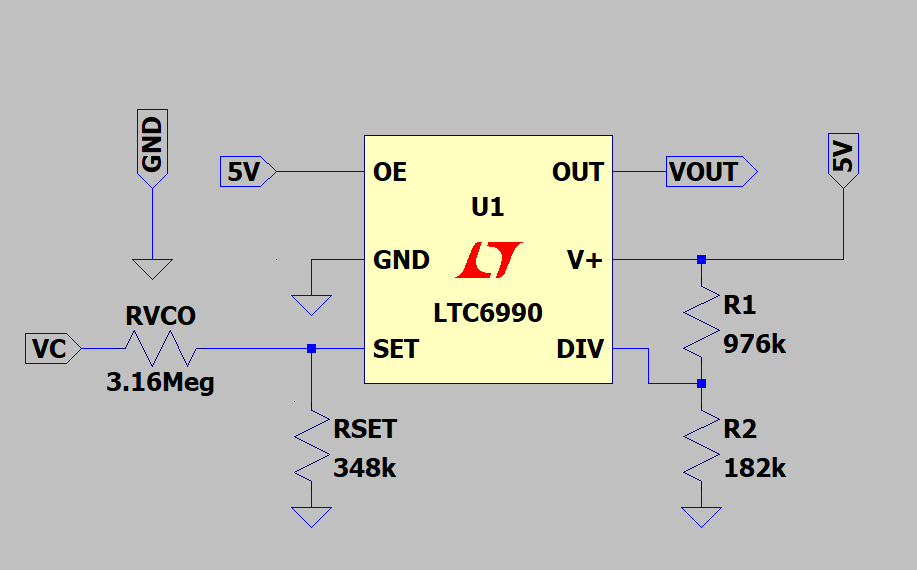
\includegraphics[width=\textwidth]{../Circuits/Images/VCO/Schematic}
    \caption{A screencap of the VCO Subcircuit}
    \label{fig:VCOSchematic}
\end{figure}

\begin{figure}[H]
    \centering 
    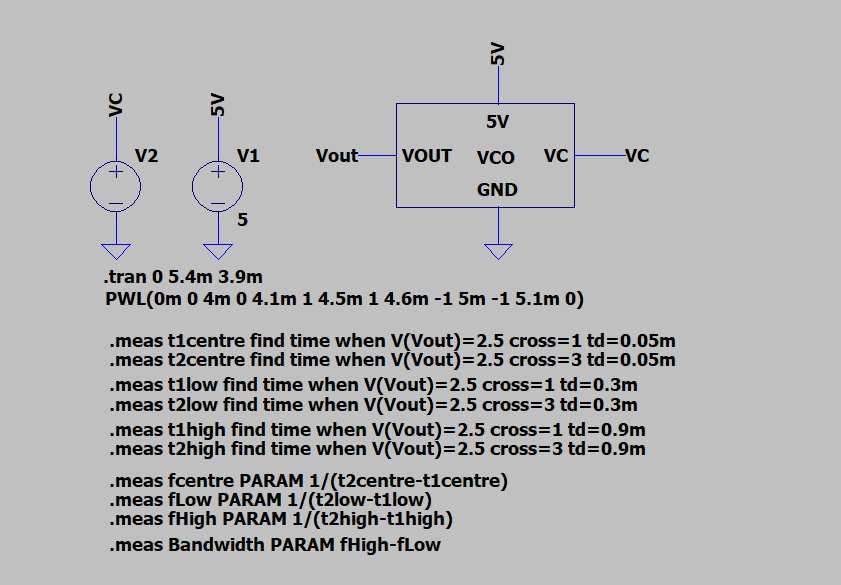
\includegraphics[width=\textwidth]{../Circuits/Images/VCO/TestBenchScreencap}
    \caption{The testbench fort the VCO Subcircuit}
    \label{fig:VCOTestBench}
\end{figure}

\begin{figure}[H]
    \centering 
    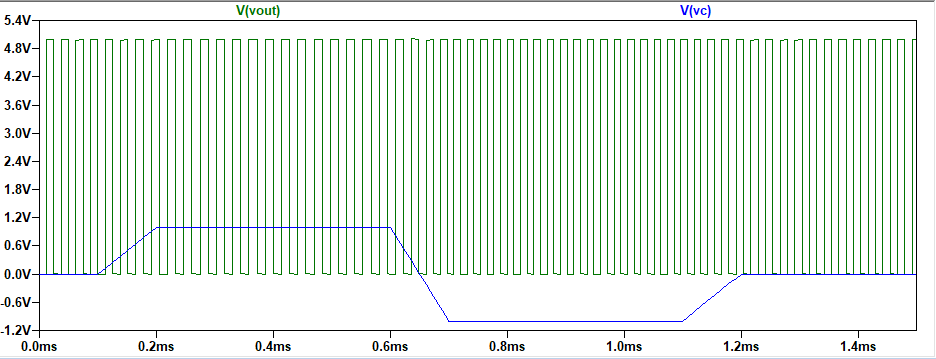
\includegraphics[width=\textwidth]{../Circuits/Images/VCO/TestBenchWaveform}
    \caption{The Waveform produced by the VCO Testbench}
    \label{fig:VCOTestBenchWaveform}
\end{figure}

\subsubsection{Transmission Amplifier}
Due to the low power requirements of the MOSFET, a SOT-23 package was chosen to conserve space and money. 
The Infineon IRLML6344\footnote{\url{https://uk.rs-online.com/web/p/mosfets/9134070/}} was used in the simulated version shown in Figure \ref{fig:TransmissionAmpSchematic} as it meets the power requirements discussed in Section \ref{sec:specificationTransmissionAmplifier} but any SOT-23 device could be used.

The testbench contains an Butterworth-Van Dyke equivalent circuit of a transducer with parameters taken from experimental data presented by \citeauthor{equivalentCircuit} in their \citeyear{equivalentCircuit} paper\cite{equivalentCircuit}.

Figure \ref{fig:TransmissionAmpTestBenchWaveform} shows the mock VCO output superimposed over the current through the resistor R1.
It shows the constant charge and discharge of the capacitor C1, demonstrating that the MOSFET is able to induce mechanical oscillation on this mock transducer.

\begin{figure}[H]
    \centering 
    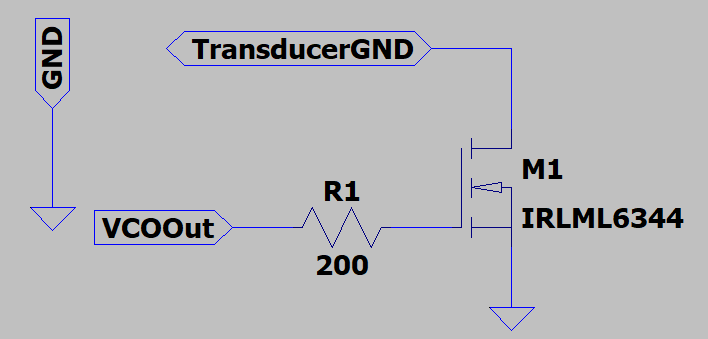
\includegraphics[width=\textwidth]{../Circuits/Images/TransmissionAmp/Schematic}
    \caption{A screencap of the Transmission Amplifier Subcircuit}
    \label{fig:TransmissionAmpSchematic}
\end{figure}

\begin{figure}[H]
    \centering 
    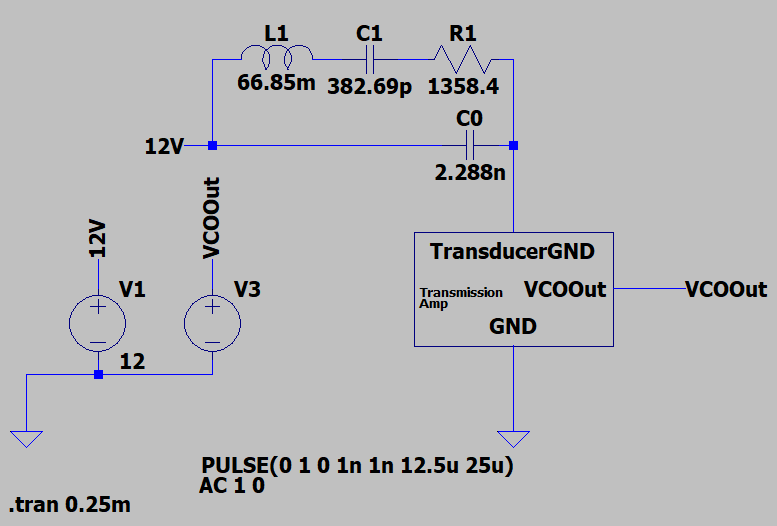
\includegraphics[width=\textwidth]{../Circuits/Images/TransmissionAmp/TestBenchScreencap}
    \caption{The testbench for the Transmission Amplifier Subcircuit}
    \label{fig:TransmissionAmpTestBench}
\end{figure}

\begin{figure}[H]
    \centering 
    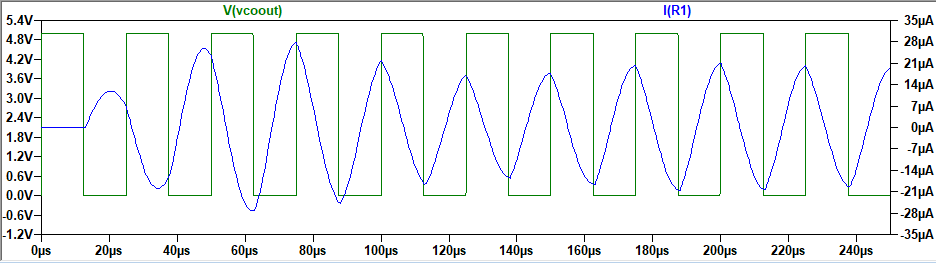
\includegraphics[width=\textwidth]{../Circuits/Images/TransmissionAmp/TestBenchWaveform}
    \caption{The Waveform produced by the Transmission Amplifier Testbench}
    \label{fig:TransmissionAmpTestBenchWaveform}
\end{figure}

\subsection{Demodulation}

\subsubsection{Pre-Amp}
The pre-amp was implemented using a non-inverting op-amp amplifier. 
This was to make setting the gain simple and to minimise costs. 
A high-speed op-amp was chosen to reproduce any of the square wave characteristics that were transmitted by the modulation stage.

Figure \ref{fig:preAmpSchematic} shows the schematic for the preamp.
The parameters for the resistances are set by the testbench.

Figure \ref{fig:preAmpTestBench} shows the test bench. 
The gain is stepped across the range given in Section \ref{sec:specificationPreAmp}.
Parameters passed to the pre-amp block for R1 and R2 are calculated as \(R1 = Rbase = 1k\Omega\) and \(R2 = Rbase \times gain\).
The input amplitude is reduced by the same factor that the gain is increased to approximate the gain of the system increasing to compensate for greater attenuation.
At each step the 3db point is calculated to give an approximation of the system bandwidth from 0 - 3db point. 
Figure \ref{fig:preAmpTestBenchOutput} shows the output of the measure directive, showing that the bandwidth requirements given in Section \ref{sec:specificationPreAmp} have been met.  

\begin{figure}[H]
    \centering 
    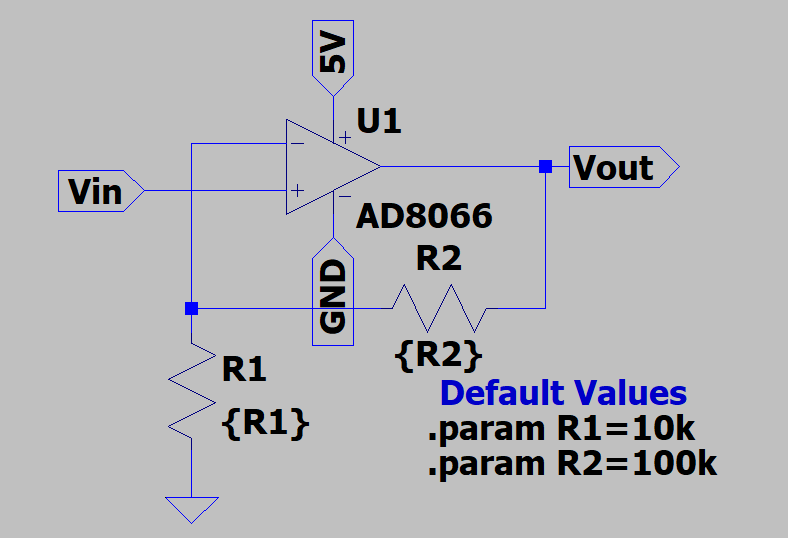
\includegraphics[width=\textwidth]{../Circuits/Images/Pre-Amp/Schematic}
    \caption{A screencap of the Pre-Amp Subcircuit}
    \label{fig:preAmpSchematic}
\end{figure}

\begin{figure}[H]
    \centering 
    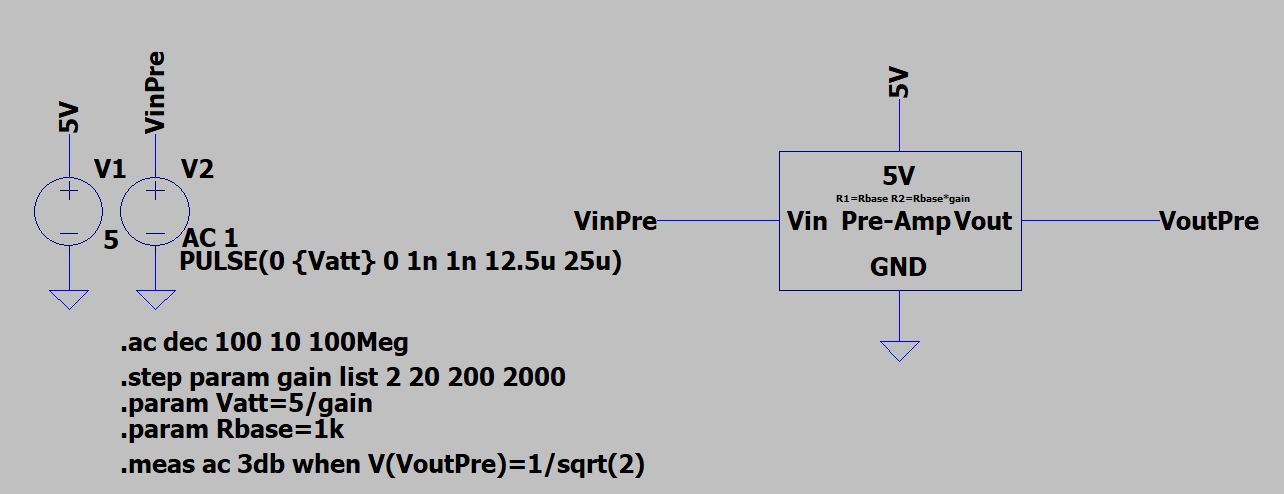
\includegraphics[width=\textwidth]{../Circuits/Images/Pre-Amp/TestBenchScreencap}
    \caption{The testbench fort the Pre-Amp Subcircuit}
    \label{fig:preAmpTestBench}
\end{figure}

\begin{figure}[H]
    \centering 
    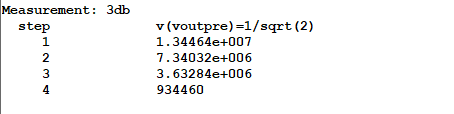
\includegraphics[width=\textwidth]{../Circuits/Images/Pre-Amp/TestBenchOutput}
    \caption{The Waveform produced by the Pre-Amp Testbench}
    \label{fig:preAmpTestBenchOutput}
\end{figure}

\subsubsection{PLL}
The TI CD4046B has been chosen to implement the PLL as it is cheap and does not require many external components. 
The ``CD4046B Phase-Locked Loop (Rev. A)'' application note was used to design the circuit\footnote{\url{https://www.ti.com/lit/an/scha002a/scha002a.pdf?&ts=1589738760062}}. 
It was not simulated in LTSpice as TI does not provide a spice model.

\begin{figure}[H]
    \centering 
    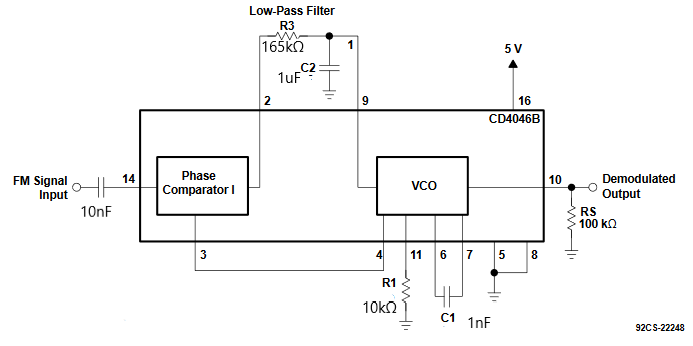
\includegraphics[width=\textwidth]{../Circuits/Images/PLL/PLLReproduction}
    \caption{The PLL subcircuiit reproduced from the example circuit.}
    \label{fig:PLLSubcircuit}
\end{figure}

Figure \ref{fig:PLLSubcircuit} contains a schematic for the PLL subcircuit reproduced from Section 4.1 of the application note. 
The passive component values have been replaced with those calculated to meet the specification presented in Section \ref{sec:specificationPLL}. 
The values are derived by following the process described in Section 4.1 of the application note. 
The VCO center frequency is set using R1 and C1 as derived from Figure 9(a).
The bandwidth, given by twice the capture frequency $f_{c}$ in the application note, was set to 8 kHz by setting $R_{3}$ and $C_{2}$ using the Equation \ref{eqn:pllBandwidth}.
The component values selected will enable the PLL to enter lock when the FM signal is received.

\begin{equation}
    \begin{split}
        2f_{c} &= \frac{1}{R_{3}C_{2}}\sqrt{\frac{2\pi f_{L}}{R_{3}C_{2}}}\\
        R_{3}C_{2}^{\frac{3}{2}} &= \frac{\sqrt{2\pi f_{L}}}{2f_{c}}
    \end{split}
    \label{eqn:pllBandwidth}
\end{equation}

With $f_{l} = f_{c} = \frac{1}{2}BW = 4 kHz$ and $C_{2} = 1 uF$:

\begin{equation*}
    \begin{split}
        R_{3}C_{2} &= 0.116s\\
        R_{3} &= 165 k\Omega
    \end{split}
\end{equation*}

\subsection{Analogue to Digital Conversion}

\subsubsection{Differentiators}
The topology for the differentiator was taken from Figure 4.69 in \citetitle{DifferentiatorTopology}\cite{DifferentiatorTopology}.
The values for the passive components were copied but this gave a gain of $\frac{1}{1000}$ so C1 was increased to 1 uF to produce the required response. 
The minimum output value was set to 0 V by adding a diode to the output of the differentiator. 
Since the differentiator output is a digital signal, the forward voltage of the diode has no impact.
To allow this diode to operate, a 1 M$\Omega$ resistor was added to the testbench output to simulate the low current drawn by a logic IC. 
The AD822 IC contains two opamps so both differentiators could be implemented using a single IC.

Figure \ref{fig:differentiatorSchematic} shows the schematic as described by \citeauthor{DifferentiatorTopology}\cite{DifferentiatorTopology}.
Figure \ref{fig:differentiatorTestBench} shows the test bench used to demonstrate the circuit. 
The input to the differentiator is driven by the triangle wave generator block as described in Section \ref{sec:implementationTriangleWaveGenerator}.
Figure \ref{fig:differentiatorTestBenchWaveform} shows the output of the differentiator. 

The differentiator produces a square wave swinging between 0 and 4.2 V.
The triangle wave is shown as well, demonstrating a clear digital signal is produced, with logic HIGH corresponding to the triangle wave ramping down, and logic LOW corresponding to the triangle wave ramping up. 
Inverting the inputs to an XOR/XNOR gate has no affect on the output signal so this inversion is not an issue. 

\begin{figure}[H]
    \centering 
    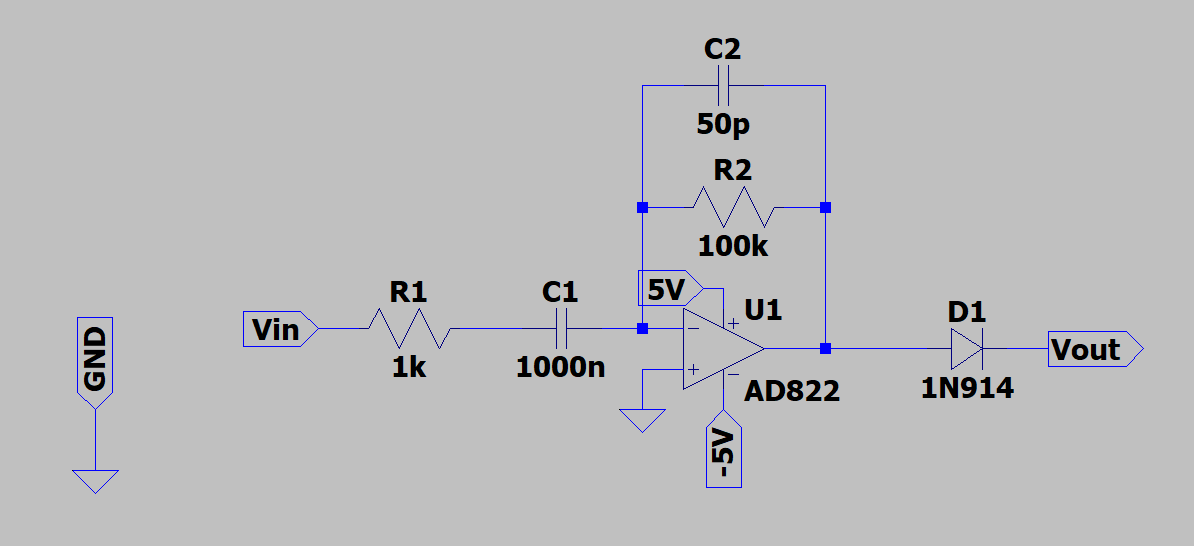
\includegraphics[width=\textwidth]{../Circuits/Images/Differentiator/Schematic}
    \caption{A screencap of the Pre-Amp Subcircuit}
    \label{fig:differentiatorSchematic}
\end{figure}

\begin{figure}[H]
    \centering 
    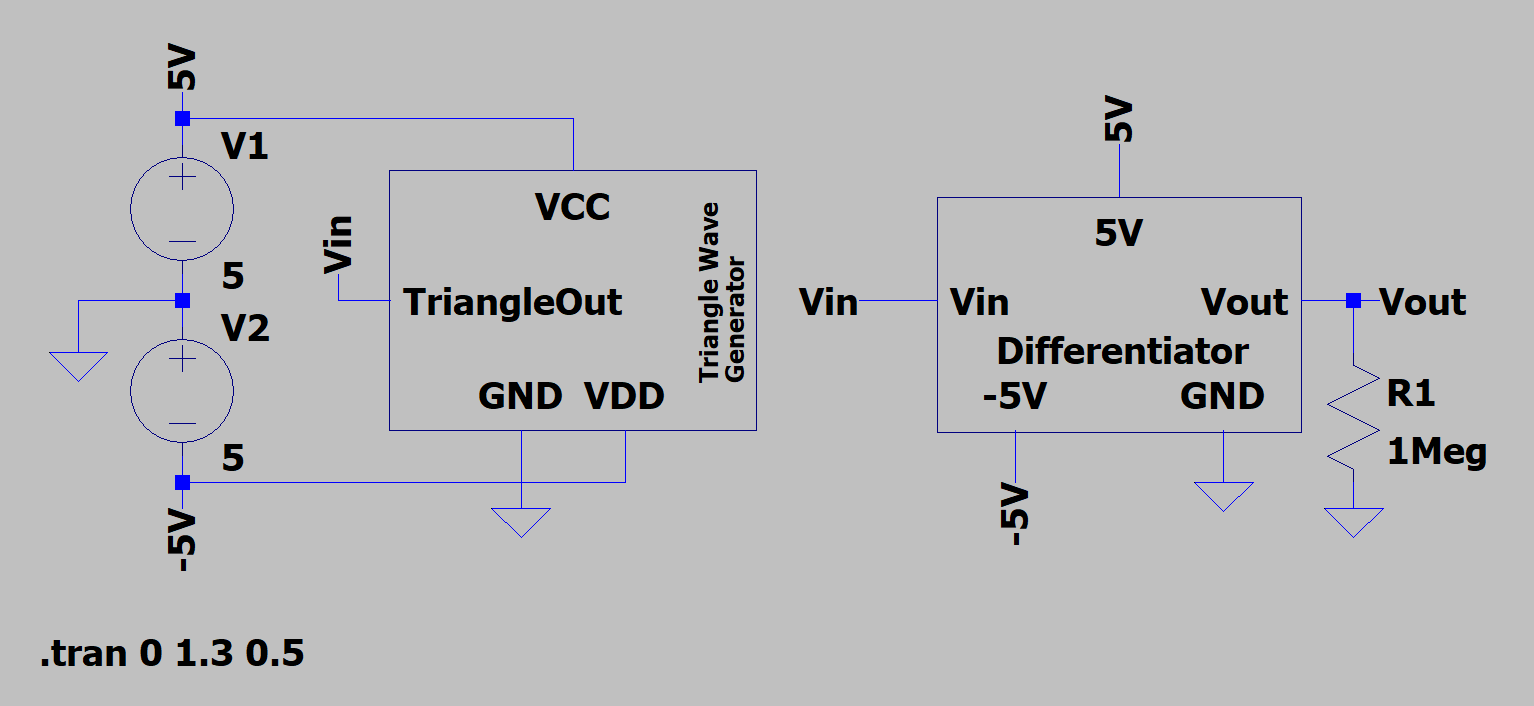
\includegraphics[width=\textwidth]{../Circuits/Images/Differentiator/TestBench}
    \caption{A screencap of the Pre-Amp Subcircuit}
    \label{fig:differentiatorTestBench}
\end{figure}

\begin{figure}[H]
    \centering 
    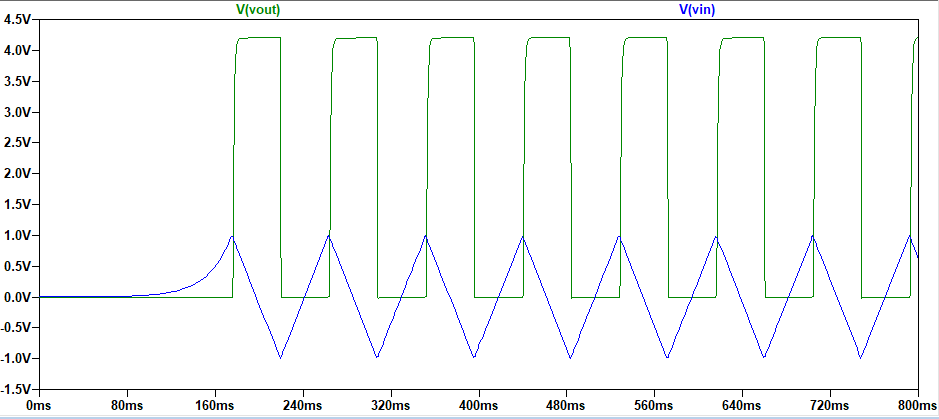
\includegraphics[width=\textwidth]{../Circuits/Images/Differentiator/TestBenchWaveform}
    \caption{A screencap of the Pre-Amp Subcircuit}
    \label{fig:differentiatorTestBenchWaveform}
\end{figure}

\subsubsection{Differential Amplifier}
The differential amplifier is split into three sections.
The first is a unity-gain inverting amplifier to remove the inversion imposed by the VCO.
The second is the LT6370 instrumentation amplifier for accurately converting the differential input to a single-ended output.
The third is a full-wave rectifier so the output signal corresponds to the \textit{magnitude} of the difference between the input signals, not the absolute difference.
The schematic is shown in Figure \ref{fig:differentialAmpSchematic}

In the event that the PLL output amplitude does not match that of the Triangle Wave Generator, the gain of the inverting amplifier can be adjusted with $R_{1}$ and $R_{2}$ so both signals are precisely matched.
The topology for the rectifier was reproduced from Figure 4.63 in \citeauthor{rectifierTopology}'s \citetitle{rectifierTopology}\cite{rectifierTopology}.
The feedback circuits of the op-amps eliminate the voltage drop across the diodes in a passive full-wave rectifier. 

Figure \ref{fig:differentialAmpTestBench} shows the Differential Amplifier testbench. 
It generates two triangle waves of equal and opposite amplitude. 
The voltage source simulating the PLL output has an increasing delay imposed on it by the step command. 
The output of the testbench is shown in Figure \ref{fig:differentialAmpTestBenchWaveform}. 
It can be seen that the maximum output voltage increases with as the delay increases. 

A simulation involving more steps was used to produce the plot in Figure \ref{fig:differentialAmpLinearity}. 
The output voltage with 0 delay is 35.3 uV.
The output voltage with the maximum delay of 14.5 ms is 3.31 V.
Figure \ref{fig:differentialAmpLinearity} shows a correlation coefficient of 0.999999959, meaning the differential amplifier easily meets the specification stated in Section \ref{sec:specificationDifferentialAmp}. 

\begin{figure}[H]
    \centering 
    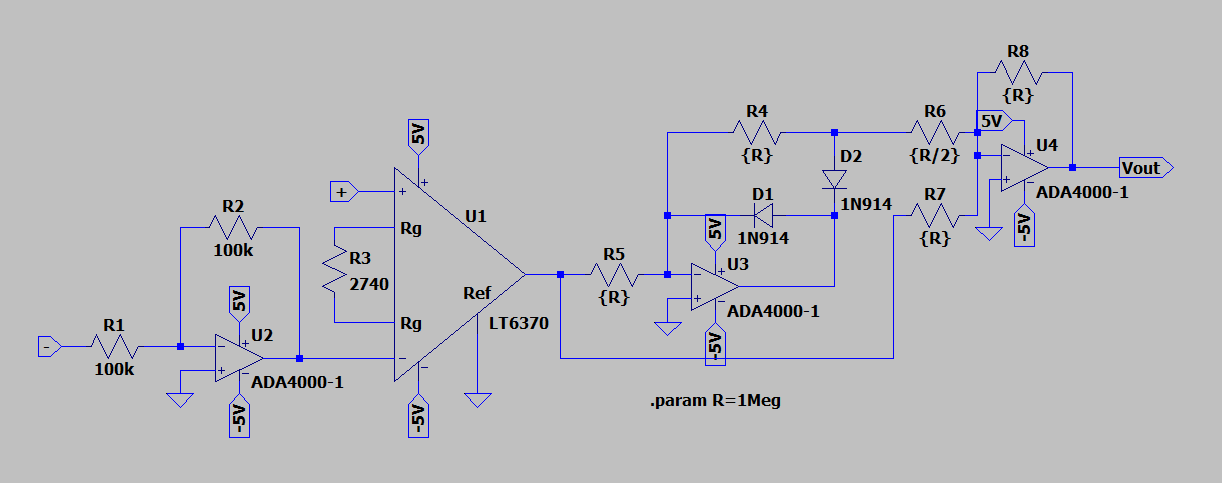
\includegraphics[width=\textwidth]{../Circuits/Images/DifferentialAmp/Schematic}
    \caption{A screencap of the Differential Amplifier Subcircuit}
    \label{fig:differentialAmpSchematic}
\end{figure}

\begin{figure}[H]
    \centering 
    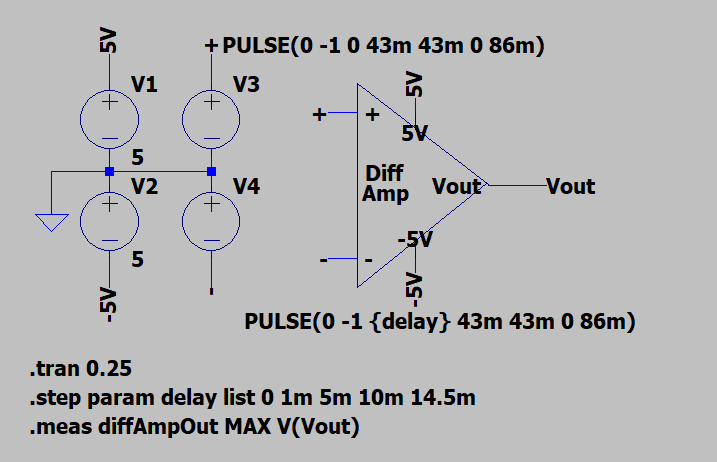
\includegraphics[width=\textwidth]{../Circuits/Images/DifferentialAmp/TestBench}
    \caption{A screencap of the Differential Amplifier Testbench}
    \label{fig:differentialAmpTestBench}
\end{figure}

\begin{figure}[H]
    \centering 
    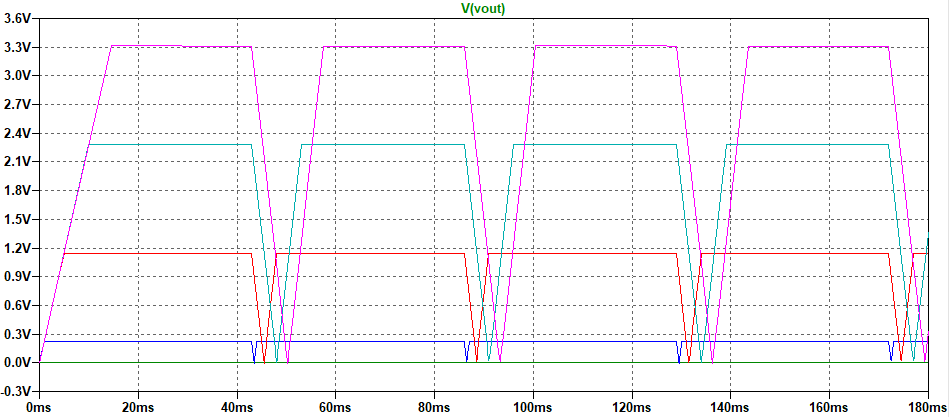
\includegraphics[width=\textwidth]{../Circuits/Images/DifferentialAmp/TestBenchWaveform}
    \caption{A screencap of the output produced by the Differential Amplifier Testbench}
    \label{fig:differentialAmpTestBenchWaveform}
\end{figure}

\begin{figure}[H]
    \centering 
    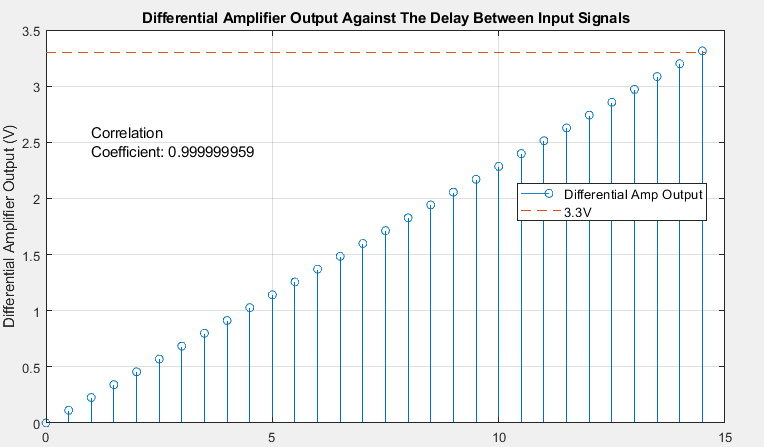
\includegraphics[width=\textwidth]{../Circuits/Images/DifferentialAmp/linearityPlot}
    \caption{A plot showing the linearity of the Differential Amplifier}
    \label{fig:differentialAmpLinearity}
\end{figure}

\subsubsection{Digital Logic}
The AD7819 should be used as the ADC.
It provides a parallel interface with with chip select and read data controls. 
The datasheet can be found here\footnote{\url{https://www.analog.com/media/en/technical-documentation/data-sheets/AD7819.pdf}}.

The microcontroller should be interfaced as shown in Figure 4 of the datasheet with the parallel interface interrupted by the 8-bit latch.
Vref should be tied to 3.3 volts through a voltage divider between 5V and GND. 
To perform a conversion, the microcontroller should follow the timing diagram as described in Figure 15 of the datasheet. 

The SN74HC573AN should be used as the 8-bit latch. 
The characteristics of this device far exceed the timing requirements of this circuit in terms of switching speed. 
The latch enable line is active HIGH so an XNOR gate should be used to generate the latch enable signal as specified in Section \ref{sec:systemWideSpecification}.

The XNOR gate should be implemented using the NC7SZ57P6X universal logic gate. 
The datasheet can be found here\footnote{\url{https://www.onsemi.com/pub/Collateral/NC7SZ58-D.PDF}}.
It is a cheap, space-friendly way to produce an XNOR gate.
It should be wired up as shown in Figure 8 of the data sheet, with connections A and B connected to the differentiator outputs and Y connected to the latch enable pin of the 8-bit latch. 
As with the latch, the characteristics of this device exceed the timing requirements of this circuit.
%
\section{Critical Analysis}
\label{sec:criticalAnalysis}%

% \printbibliography

\end{document}